\documentclass[11pt, letterpaper]{article}
\setlength{\parindent}{0in}
\setlength{\textheight}{8.7in}
\setlength{\textwidth}{6.8in}
\setlength{\oddsidemargin}{-0.3in}
\setlength{\evensidemargin}{0.0in}
\addtolength{\topmargin}{-1in}
\setlength{\parskip}{0.1in}

\usepackage{amsmath, amsfonts, color}
\usepackage{bm}
\usepackage{booktabs}
\usepackage{enumerate}
\usepackage{graphicx}
\usepackage{multirow}
\usepackage{pdfpages}
\usepackage{placeins}
\newcommand*{\justifyheading}{\raggedleft}


\renewcommand{\baselinestretch}{1.0}

\newcommand{\bx}{{\bm x}}
\newcommand{\bX}{{\bm X}}
\newcommand{\by}{{\bm y}}
\newcommand{\bY}{{\bm Y}}
\newcommand{\bW}{{\bm W}}
\newcommand{\bG}{{\bm G}}
\newcommand{\bR}{{\bm R}}
\newcommand{\bZ}{{\bm Z}}
\newcommand{\bV}{{\bm V}}
\newcommand{\bL}{{\bm L}}
\newcommand{\bz}{{\bm z}}
\newcommand{\be}{{\bm e}}
\newcommand{\bgamma}{{\bm \gamma}}
\newcommand{\bbeta}{{\bm \beta}}
\newcommand{\balpha}{{\bm \alpha}}
\newcommand{\bSigma}{{\bm \Sigma}}
\newcommand{\bmu}{{\bm \mu}}
\newcommand{\btheta}{{\bm \theta}}
\newcommand{\bepsilon}{{\bm \epsilon}}
\newcommand{\bone}{{\bm 1}}
\newcommand{\bzero}{{\bm 0}}
\newcommand{\bC}{{\bm C}}
\newcommand{\bI}{{\bm I}}
\newcommand{\bA}{{\bm A}}
\newcommand{\bB}{{\bm B}}
\newcommand{\bQ}{{\bm Q}}
\newcommand{\bS}{{\bm S}}
\newcommand{\bD}{{\bm D}}
\newcommand{\cQ}{\mathcal{Q}}
\newcommand{\cU}{\mathcal{U}}
\newcommand{\cI}{\mathcal{I}}
\newcommand{\cL}{\mathcal{L}}

\newcommand{\beas}{\begin{eqnarray*}}
\newcommand{\eeas}{\end{eqnarray*}}

\newenvironment{equationarrayright}{
                          \begin{eqnarray*}
                          \begin{array}{rcll}
                         }{
                          \end{array}
                          \end{eqnarray*}
                         }
\newcommand{\bear}{\begin{equationarrayright}}
\newcommand{\eear}{\end{equationarrayright}}


\DeclareMathOperator*{\argmin}{arg\,min}

\title{STAT/BIOST 571: Homework 8}
\author{Philip Pham}
\date{\today}

\begin{document}

\maketitle

\section*{Problem 1: GEE and GLMM; interpretation of marginal parameters in logistic regression models; missing data (20 points)}
 
{\em Download the \texttt{fluoride.csv} dataset from the course website.  This dataset contains 3846 observations of fluoride intake for 1279 children, with follow-ups at ages 1.5, 3, 6, and 9 months, but with some observations missing for individual children.  The variable $id$ indexes unique children, $age$ denotes age in months, $income$ is an indicator for maternal income over 30 thousand dollars per year, $fluoride$ is total 
fluoride intake (mg per kg of body weight), and $fl$ is an indicator for $fluoride > 0.05$.
Our primary interest is the relationship between the binary outcome $fl$ and the child's age, potentially
including effect modification by maternal income.  We will fit logistic regression models for the $fl$ outcome with the 
standard mean variance relationship and either a multiplicative interaction 
\begin{equation}
\label{eq:interact}
\mu=expit(\beta_0 + \beta_1 \times age + \beta_2 \times income + \beta_3 \times age \times income)
\end{equation}
or just an intercept and a main effect 
\begin{equation}
\label{eq:nointeract}
\mu=expit(\beta_0 + \beta_1 \times age). 
\end{equation}
In all analyses, we account for correlation within children and assume the data from different children are independent.}
\begin{enumerate}[(a)]
{\em \item  Fit model~(\ref{eq:interact}) using GEE with independence and exchangeable working
correlation models and using a standard GLMM with random intercepts.  Report point estimates and standard error estimates 
for all four regression coefficients and all three model fits in a single table (use robust standard errors for GEE and model-based versions for GLMM).}

\begin{table}[ht]
  \scriptsize
  \centering
  \begin{tabular}{lrrrrrr}
\toprule
Correlation Structure & \multicolumn{2}{c}{GEE Independent} & \multicolumn{2}{c}{GEE Exchangeable} & \multicolumn{2}{c}{Mixed Model} \\
{} &        Estimate & Standard Error &         Estimate & Standard Error &    Estimate & Standard Error \\
Coefficient            &                 &                &                  &                &             &                \\
\midrule
(Intercept), $\beta_0$ &        0.576457 &       0.117464 &         0.524520 &       0.115018 &    1.171506 &       0.208960 \\
age, $\beta_1$         &       -0.048729 &       0.017763 &        -0.023578 &       0.017634 &   -0.054638 &       0.029439 \\
income, $\beta_2$      &       -0.964447 &       0.148575 &        -0.944916 &       0.145484 &   -2.083890 &       0.269759 \\
age:income, $\beta_3$  &        0.076834 &       0.022462 &         0.061876 &       0.022088 &    0.131501 &       0.036506 \\
\bottomrule
\end{tabular}

  \caption{Model fits of Equation \ref{eq:interact} with different correlation
    structures to the data in \texttt{fluoride.csv}.}
  \label{tab:model_interaction_full_data_fit}
\end{table}

\begin{description}
\item[Solution:] The estimates and standard errors can be found in Table
  \ref{tab:model_interaction_full_data_fit}. Robust sandwich estimates were used
  for standard errors in the GEE model. For the Mixed Model correlation
  structure with random intercepts, model-based standard errors were used.

  Code to fit the models is found in the Appendix.
\end{description}
{\em \item Discuss any differences between the estimated values of $\beta_1$ from your three fitted models.}
{\em \item For each of your three fitted models, write a short paragraph summarizing your main findings.  Specifically, give scientifically interpretable statements (including confidence intervals) about the relationships between fluoride intake and age
in children with maternal income greater than 30 thousand dollars per year and
in children with maternal income less than 30 thousand dollars per year.}
{\em \item Now repeat part (a), but use model~(\ref{eq:nointeract}) instead of~(\ref{eq:interact}) (there are now only two regression coefficients to report per model).}
{\em \item Download the dataset \texttt{fluoride.miss.csv} from the course website and repeat the calculations from part (d).  Note \texttt{fluoride.miss.csv} is a subset of \texttt{fluoride.csv}, with more missing data.}
{\em \item  Discuss the differences between your results in parts (d) and (e).  Speculate
about the missingness mechanism that gave rise to the \texttt{fluoride.miss.csv} dataset and 
explain how this might account for what you observe.  You might find it
helpful to conduct exploratory analyses of the two datasets and to consider your findings from part (a) of
this problem.
}

\end{enumerate}


\FloatBarrier

\section*{Appendix}

Code to fit the models is attached on the following pages.

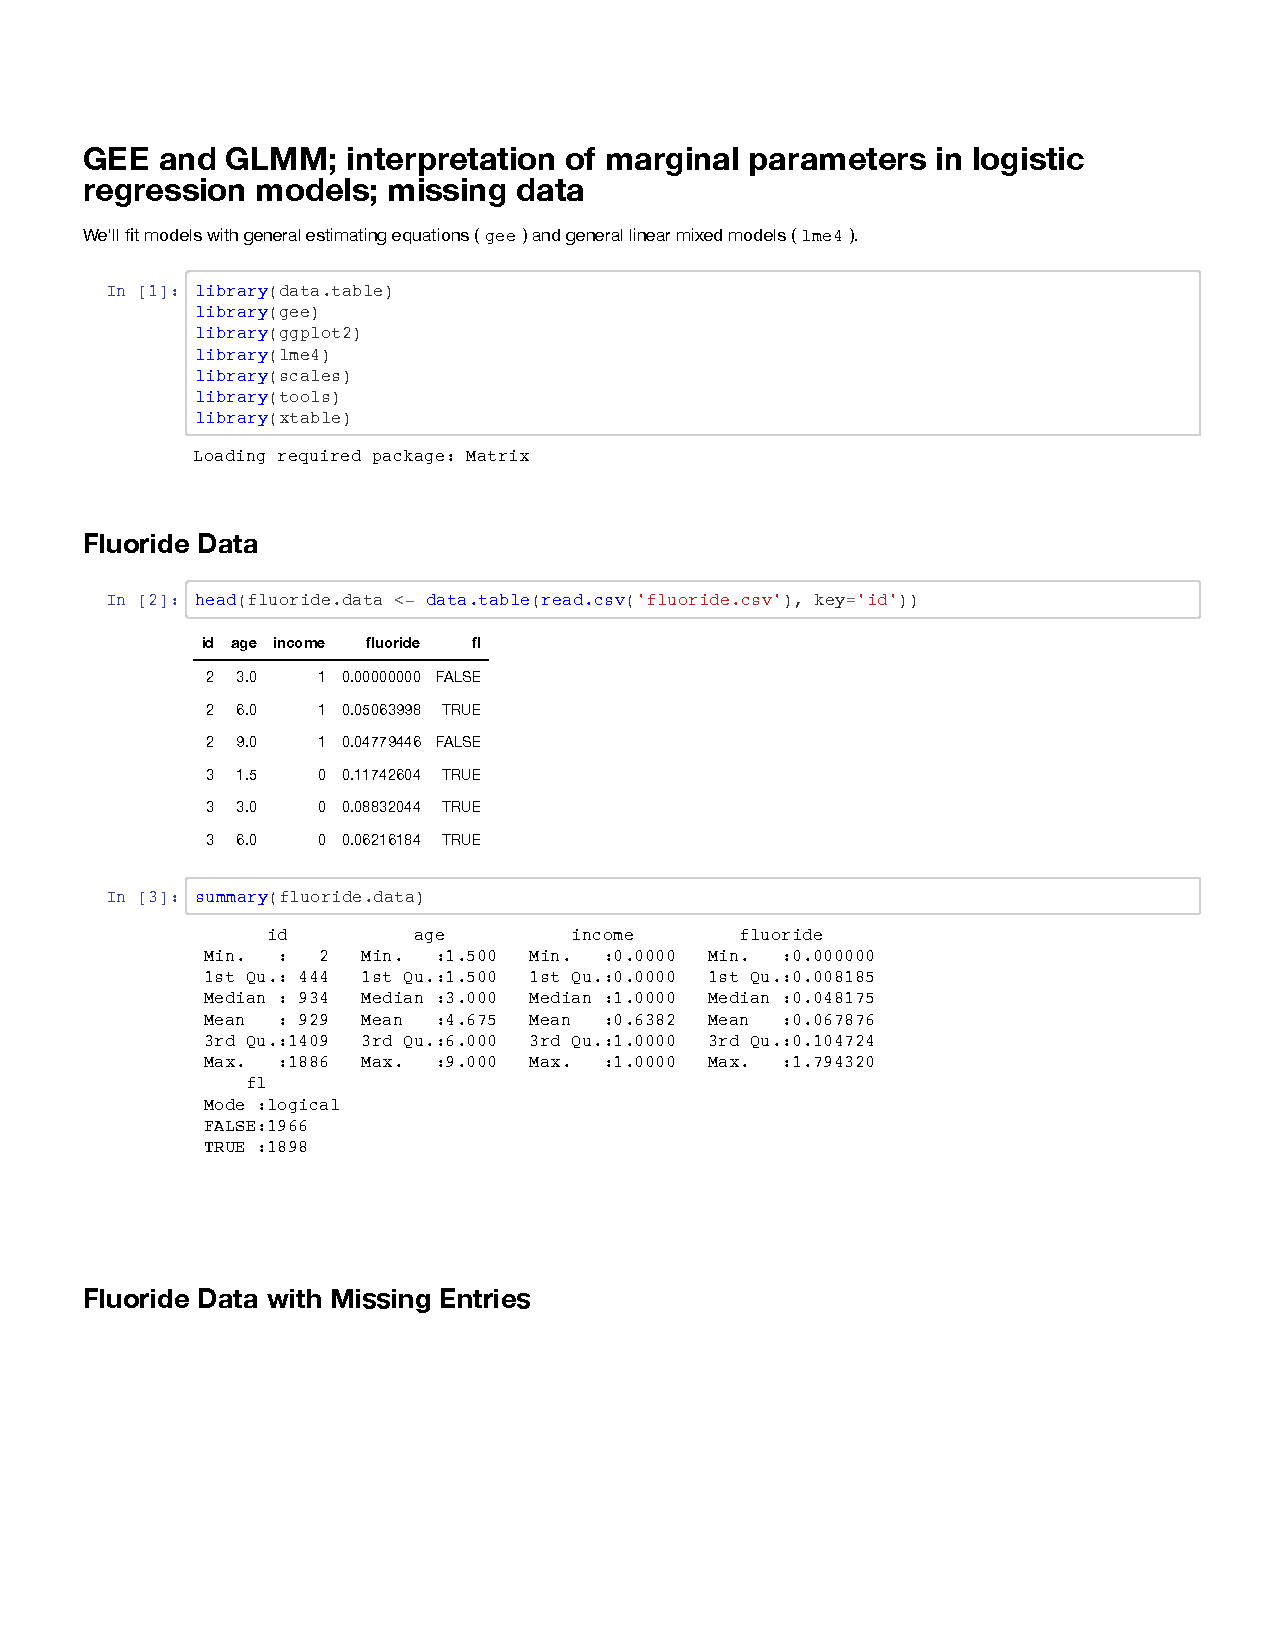
\includepdf[pages=-]{flouride.pdf}

\end{document}

